%&latex
\fancyhead[RO,LE]{\thepage}
\fancyfoot{} 
\chapter{Introduction}

\section{Problem Statement}

\emph{Segmentation} is the task of identifying regions in images  with related content. Given the ease with which humans can segment images, it is easy to forget how challenging it has been to develop computer segmentation algorithms that can match segmentations produced by humans. Indeed, even though
"image segmentation is one of the oldest and most widely studied problems"~\cite{Szeliski-2010} in computer vision, "there still exists a wide gap between automated and human segmentation performance"~\cite{Szeliski-2010}.

%*******************************************************************************
% FIGURE Segmentation
\begin{figure}[t]
\centering
\subfigure[a scene from the Berkeley Segmentation Dataset]{
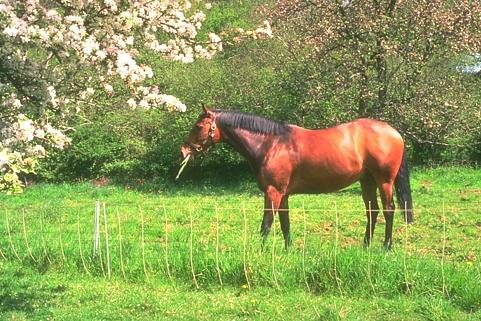
\includegraphics[width=3.5in]{figures/segmentation-scene.jpg}
}
\subfigure[human segmentations of the same scene]{
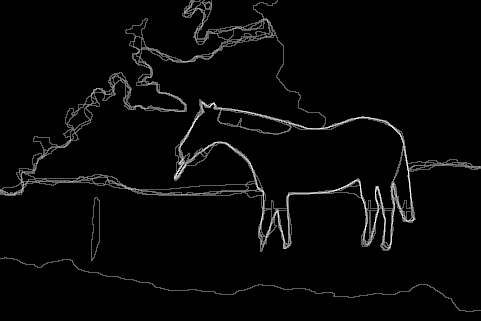
\includegraphics[width=3.5in]{figures/human-segmentations.png}
}
\subfigure[an automated segmentation of the same scene using local image properties (brightness and texture gradients); we see that the automated segmentation fails to capture the holistic understanding of the scene shown in the human segmentations in (b)]{
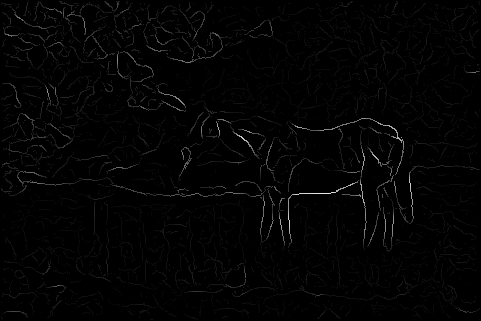
\includegraphics[width=3.5in]{figures/automated-segmentations.png}
}
\caption{Human and automated segmentation performance on an image from the Berkeley Segmentation Dataset~\cite{Martin-2001}.}
\label{fig:segmentation}
\end{figure}
%*******************************************************************************

Image segmentation is challenging because determining if two pixels in an image "go together"~\cite{Szeliski-2010} often requires an abstract and holistic understanding of the image, and in general it is difficult for computer algorithms to gain this understanding. Analyzing local image features such as edges and contours, as well as local image properties such as color and texture is not guaranteed to capture the relevant relationships between pixels (see Figure \ref{fig:segmentation}). Determining the mixture of image properties required to capture such relationships remains an active area of research.

%*******************************************************************************
% FIGURE Medical Image
\begin{figure*}[t]
\centering
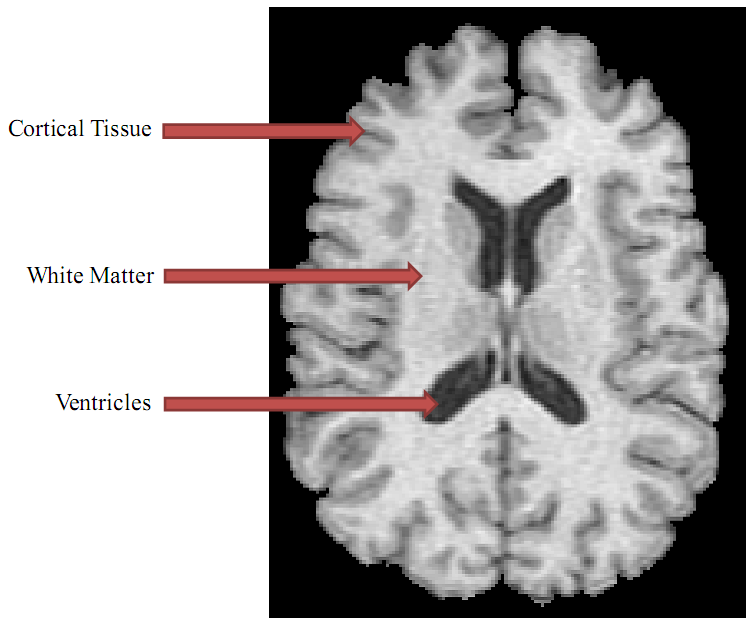
\includegraphics[width=6.0in]{figures/medical-image-with-labels.png}
\caption{A typical 2D cross-sectional magnetic resonance image of a brain. Distinct structures are apparent (labelled with red arrows for additional clarity) but boundaries are not precisely defined~\cite{Pham-1999}.}
\label{fig:medical-image}
\end{figure*}
%*******************************************************************************
%*******************************************************************************
% FIGURE Medical Image
\begin{figure*}[t]
\centering
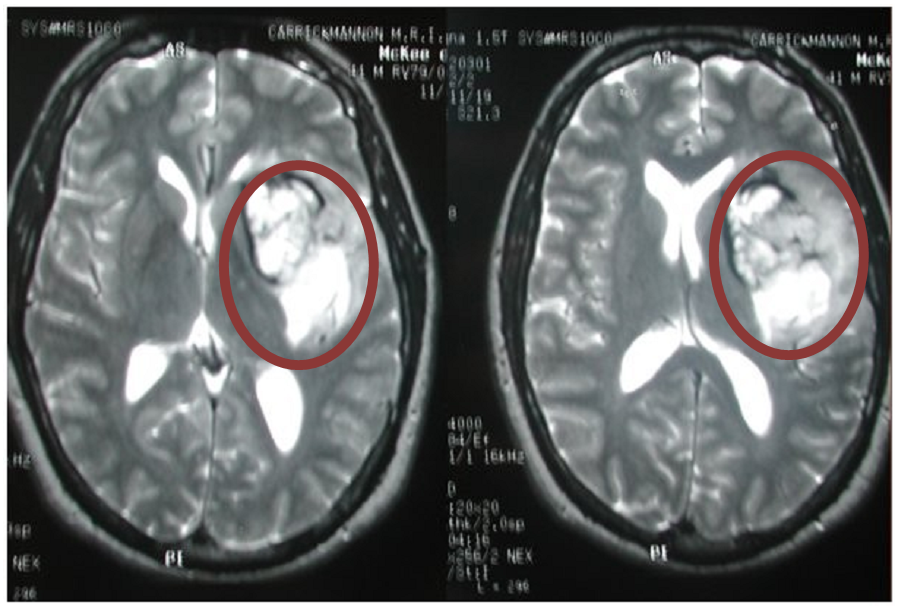
\includegraphics[width=6.0in]{figures/brain-tumour-with-labels.png}
\caption{A 2D cross-sectional magnetic resonance image of a brain with a visible brain tumour. The tumour (approximately outlined in red) is heterogeneous and not precisely defined~\cite{Botchu-2005}.}
\label{fig:brain-tumour}
\end{figure*}
%******************************************************************************
Image segmentation is particularly important in diagnostic medicine. The use of medical scanning equipment to acquire 3D images of the human body is commonplace. These images must be carefully segmented into meaningful regions before they can be be quantified and analyzed for the purposes of diagnosis and treatment planning. For example, there is no single treatment for cancer which is most effective for treating all sizes of tumour. In other words, for different sizes of tumour, there are different treatment methods which offer optimal patient outcomes. To determine the optimal treatment for a particular cancer patient, a physician must often segment a tumour from a medical image to accurately determine its size.

Physicians often resort to very crude approximations when segmenting large 3D medical images since precise manual segmentation of these images is such a slow process. This practice may result in sub-optimal patient outcomes in cases where the physician's segmentation exhibits large approximation error.

In the medical imaging domain, image segmentation is especially challenging since current medical scanning equipment may introduce noise and non-linearly distributed image intensity distortions into the resulting medical images. Moreover, medical images typically lack precisely defined intensity boundaries at physical tissue boundaries (see Figure \ref{fig:medical-image}).

Threshold-based flood-fill techniques~\cite{Chen-2008} can compute  segmentation results very quickly but often fail when the region-of-interest (ROI) is heterogeneous~\cite{Unger-2008}. This makes it difficult to segment some  structures, like brain tumors, which have variable intensity, texture, shape and size~\cite{Chen-2008} (see Figure \ref{fig:brain-tumour}). Computer-assisted level set segmentation techniques~\cite{Lefohn-2003-MICCAI,Cates-2004} have been shown to produce accurate segmentations and reduce the variability of difficult segmentation tasks in medical imaging. The level set method is a powerful, flexible, and accurate numerical technique for image segmentation under challenging conditions since the segmentation process can depend on image properties (e.g. color or texture) and can enforce geometric constraints on the segmented regions (e.g. smoothness).

The level set method begins with an implicitly represented seed surface embedded within a regular scalar grid. The level set method deforms this surface to envelop a corresponding region-of-interest (ROI) in the original image by iteratively solving a partial differential equation defined at each grid element. This method typically requires thousands of iterations to converge and there can be millions of grid elements that must be updated during each iteration. The level set method has historically resulted in long computation times and therefore limited clinical utility.

In response to the demand for faster level set segmentation methods, researchers have developed significantly accelerated algorithms for solving the level set equations~\cite{Whitaker-1994, Adalsteinsson-1995,Peng-1999,Lefohn-2003-Vis,Lefohn-2003-MICCAI,Lefohn-2004,Cates-2004,Jeong-2009}. These algorithms are motivated by the observation that computations can be avoided in regions that are far away from the level set surface without affecting the resulting segmentation. Leveraging this insight, previous algorithms maintain dynamic data structures to represent the \emph{active computational domain} -- the grid elements that must be updated during each iteration. There is significant spatial coherence among these grid elements since they are all near the level set surface.
The fastest algorithms leverage the general-purpose and massively parallel computational power of commodity graphics processing units (GPUs). These parallel GPU algorithms~\cite{Lefohn-2003-Vis,Lefohn-2003-MICCAI,Lefohn-2004,Cates-2004,Jeong-2009} are motivated by the observation that within each iteration, the solution of the level set equations at each grid element is independent from the solution at each other grid element. Therefore the solutions for every grid element can be computed in parallel on the many computational cores of the GPU. However, the previous state-of-the-art GPU algorithm I test in this thesis took over 100 seconds  to converge  on  the  white and grey matter in a $256^3$ medical image of a human head, even when running on a state-of-the-art GPU. The fastest level set segmentation algorithms are still too slow. This limitation constrains clinical applications and motivates the research herein.

In this thesis I present a novel GPU level set segmentation algorithm that dramatically improves computational efficiency without sacrificing segmentation accuracy. In a series of controlled experiments using noisy magnetic resonance images (MRIs) generated from the BrainWeb Simulated Brain Database~\cite{BrainWeb-2010,Kwan-1996,Cocosco-1997,Collins-1998,Kwan-1999}, I demonstrate that my algorithm reduces the total number of processed grid elements by $16 \times$ and converges $14 \times$ faster than previous state-of-the-art GPU algorithms~\cite{Lefohn-2003-Vis,Lefohn-2003-MICCAI,Lefohn-2004,Cates-2004} with equal accuracy in all experiments. My algorithm runs entirely on the GPU without requiring any additional data processing on the CPU, thereby enabling interactive 3D visualization and real-time control of the evolving segmentation.

\section{Assumptions}

Given the acknowledged difficulty of fully automated image segmentation, researchers have focused on easier sub-problems in order to obtain results that are competitive with human segmentations~\cite{Szeliski-2010}. In this thesis I tackle a simpler sub-problem of the more general image segmentation problem by making the following assumptions:

\begin{itemize}

    \item I assume that my algorithm is only concerned with generating binary (i.e. foreground and background) segmentations. This assumption is motivated by a common workflow in the medical community: segmenting a region-of-interest (ROI) from a medical image for subsequent analysis.

    \item I assume that my algorithm is guided by user interaction. This assumption is motivated by a common preference the medical community: physicians often prefer intuitive interactive segmentation methods over fully automated methods~\cite{Unger-2008} since interactive methods allow them to drive the segmentation process according to their domain expertise. This expertise would be difficult to distill into a fully automated method.

    \item I assume that there is some difference in image intensity between foreground and background objects. Moreover I assume that this difference approximately exceeds the heterogeneity of the foreground objects being segmented and the noise in the image. Previous state-of-the-art GPU level set segmentation algorithms~\cite{Lefohn-2003-Vis,Lefohn-2003-MICCAI,Lefohn-2004,Cates-2004,Jeong-2009} also make this assumption as it simplifies the solution of the level set equations. In practice this assumption does not always hold, and therefore it introduces a limitation that my algorithm shares with previous GPU algorithms~\cite{Lefohn-2003-Vis,Lefohn-2003-MICCAI,Lefohn-2004,Cates-2004,Jeong-2009}. This assumption could be relaxed with a more intelligent accounting of image properties when solving the level set equations. However this is not the focus of my research. Instead I am focused on developing optimizations that are orthogonal to the accounting of image properties used when solving the level set equations. The optimizations that I present in this thesis are compatible with a wide variety of image properties and features. 
\end{itemize}

\section{Contributions and Results}

This thesis makes the following contributions:

\begin{itemize}

    \item A novel algorithm for limiting the active computational domain to the minimal set of changing level set grid elements by leveraging both spatial and temporal coherence in the active computational domain;

    \item A formal derivation of the above algorithm;
    
    \item A novel mapping of this algorithm to massively parallel GPU hardware. This GPU algorithm scales efficiently to an unbounded number of parallel processors while performing asymptotically no more work than the most efficient sequential algorithm, and does so in asymptotically fewer steps. This GPU algorithm does not require any additional data processing on the CPU, thereby enabling smooth interactive 3D visualization and real-time control of the evolving segmentation;

    \item A\ formal proof of the above GPU algorithm's asymptotic properties;
and
    \item A series of controlled experiments using noisy magnetic resonance images (MRIs) generated from the BrainWeb Simulated Brain Database~\cite{BrainWeb-2010,Kwan-1996,Cocosco-1997,Collins-1998,Kwan-1999}. I demonstrate significant performance benefits over previous state-of-the-art parallel algorithms~\cite{Lefohn-2003-MICCAI,Lefohn-2003-Vis,Cates-2004,Lefohn-2004}. I demonstrate that my algorithm: reduces the total number of processed level set field elements by $16 \times$ and converges $14 \times$ faster than previous state-of-the-art parallel algorithms; converges $685 \times$ faster than previous sequential algorithms; and produces equally accurate segmentations to previous parallel algorithms with less than 0.2\% variability in all experiments.



\end{itemize}

\section{Thesis Overview}

The remainder of this thesis is organized as follows. In Chapter \ref{chapter:background} I describe the technical background and related work most relevant to my research. I discuss an emerging research field that seeks to accelerate general-purpose parallel computations by performing them on GPUs. I describe the current state-of-the-art GPU algorithms for level set segmentation. I show that previous algorithms maintain a sparse active computational domain that is coherent in space only.

In Chapter \ref{chapter:temporal} I present a new algorithm for maintaining a sparse active computational domain for solving the level set equations that is coherent in both space and time. I provide the intuitive motivation for this algorithm, a discussion of the underlying mathematics, and sequential psuedo-code for clarity.

In Chapter \ref{chapter:parallel} I discuss the challenges associated with parallelizing the algorithm described in the previous chapter. I present a massively parallel algorithm that overcomes these challenges and I discuss an implementation of this algorithm on a commodity GPU.

In Chapter \ref{chapter:evaluation} I describe a methodology for evaluating the parallel algorithm from the previous chapter. I analyze the asymptotic performance and memory efficiency of this algorithm, and describe a series of experiments that compares the computational efficiency and accuracy of my GPU algorithm to a previous state-of-the-art GPU algorithm. The results of these experiments show that my algorithm significantly outperforms the previous state-of-the-art algorithm with no reduction in segmentation accuracy.

In Chapter \ref{chapter:conclusions} I propose future research directions that build on the work presented in this thesis.


